\documentclass[11pt]{article}
\usepackage[utf8]{inputenc}
\usepackage[margin=0.85in]{geometry}
\usepackage{xcolor}
\usepackage{titlesec}
\usepackage{graphicx}
\usepackage{courier}
\usepackage{tikz}
\usepackage{float}
\usetikzlibrary{shapes.geometric, arrows.meta, positioning}

\definecolor{nodefill}{RGB}{230,240,250}

\titleformat{\section}{\normalsize\bfseries}{}{0em}{}[\titlerule]
\titlespacing*{\section}{0pt}{1ex plus 0.5ex minus .2ex}{0.3ex plus .2ex}

\begin{document}

\begin{center}
\textbf{Project Demo} \\
COM S 5130 \quad Uneeb Kamal, Talha Hassan
\end{center}

\section{Queries}

\textbf{Call Graph:} ``Which functions can reach encode?'' --- Find transitive callers.\\
\textbf{Coverage:} ``Show functions with branch coverage below 80\%.'' --- Identify under-tested code.\\
\textbf{Data Flow:} ``What is the data flow from main:freq?'' --- Track inter-procedural dependencies.\\
\textbf{Metrics:} ``Which functions have the most instructions?'' --- Locate hot spots.

\begin{figure}[H]
\centering
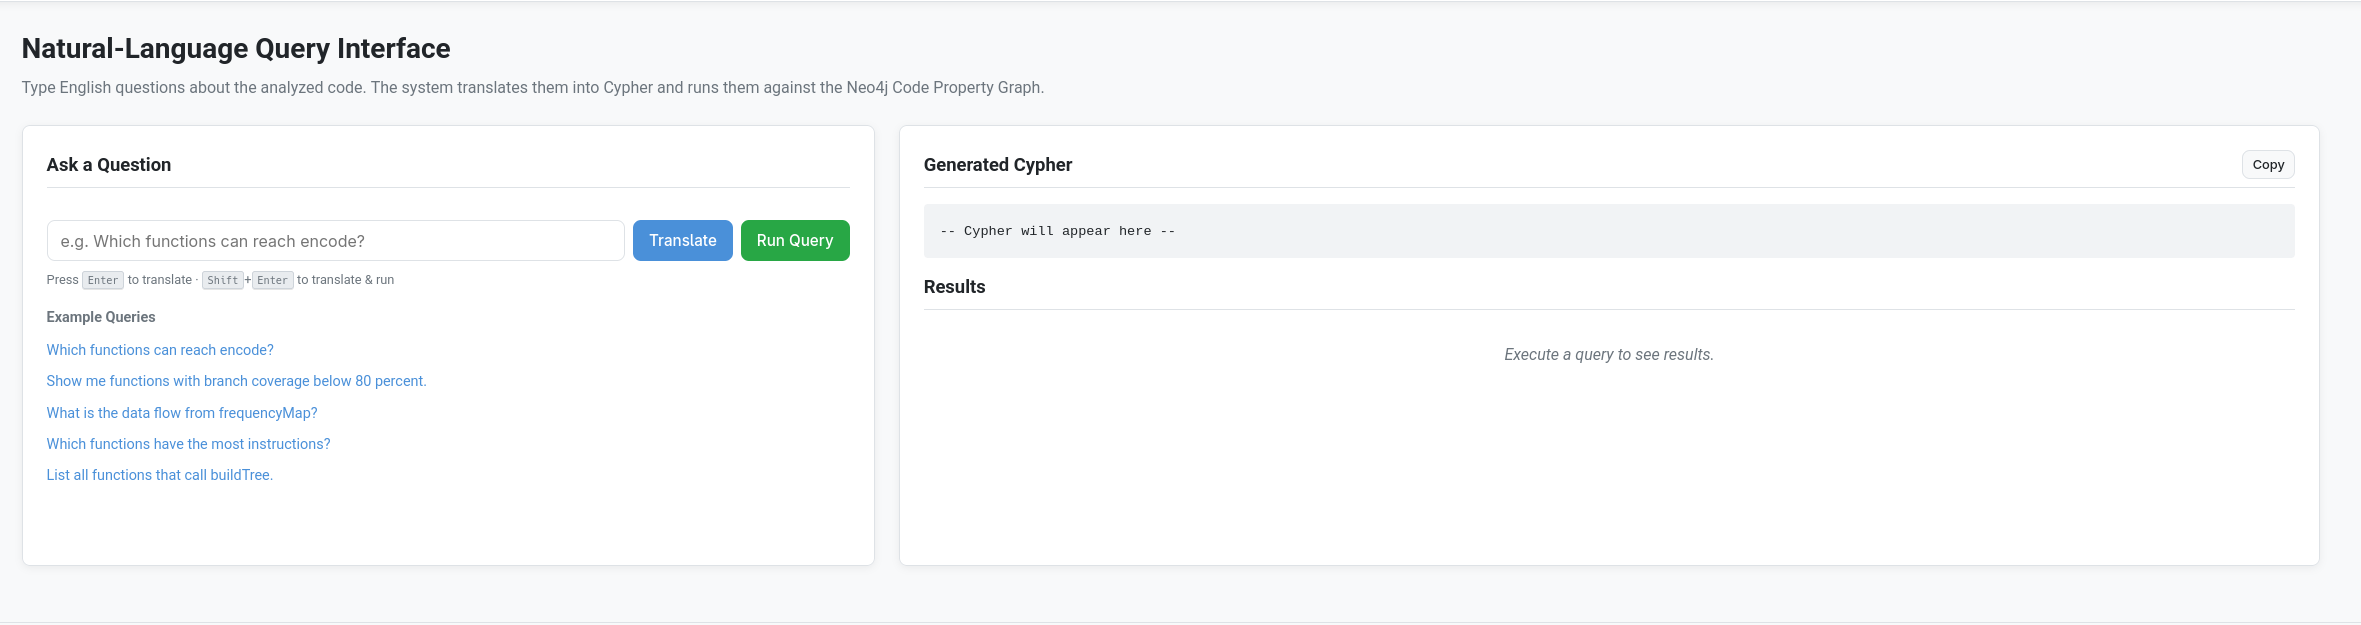
\includegraphics[width=0.95\textwidth]{screenshots/screen_query_interface.png}
\end{figure}

\section{Workflow}

\begin{figure}[H]
\centering
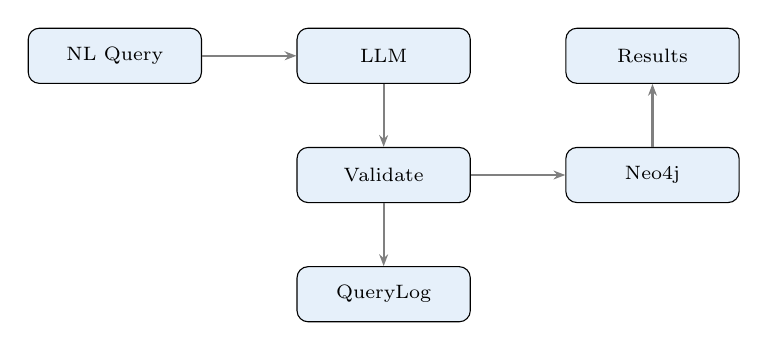
\begin{tikzpicture}[
  node distance=0.8cm and 1.2cm,
  box/.style={rectangle, draw, fill=nodefill, rounded corners, minimum width=2.2cm, minimum height=0.7cm, align=center, font=\scriptsize},
  arrow/.style={-{Stealth[length=1.5mm]}, thick, gray},
]
\node[box] (u) {NL Query};
\node[box, right=of u] (l) {LLM};
\node[box, below=of l] (v) {Validate};
\node[box, right=of v] (n) {Neo4j};
\node[box, above=of n] (d) {Results};
\node[box, below=of v] (s) {QueryLog};
\draw[arrow] (u) -- (l); \draw[arrow] (l) -- (v);
\draw[arrow] (v) -- (n); \draw[arrow] (n) -- (d);
\draw[arrow] (v) -- (s);
\end{tikzpicture}
\end{figure}

\begin{figure}[H]
\centering
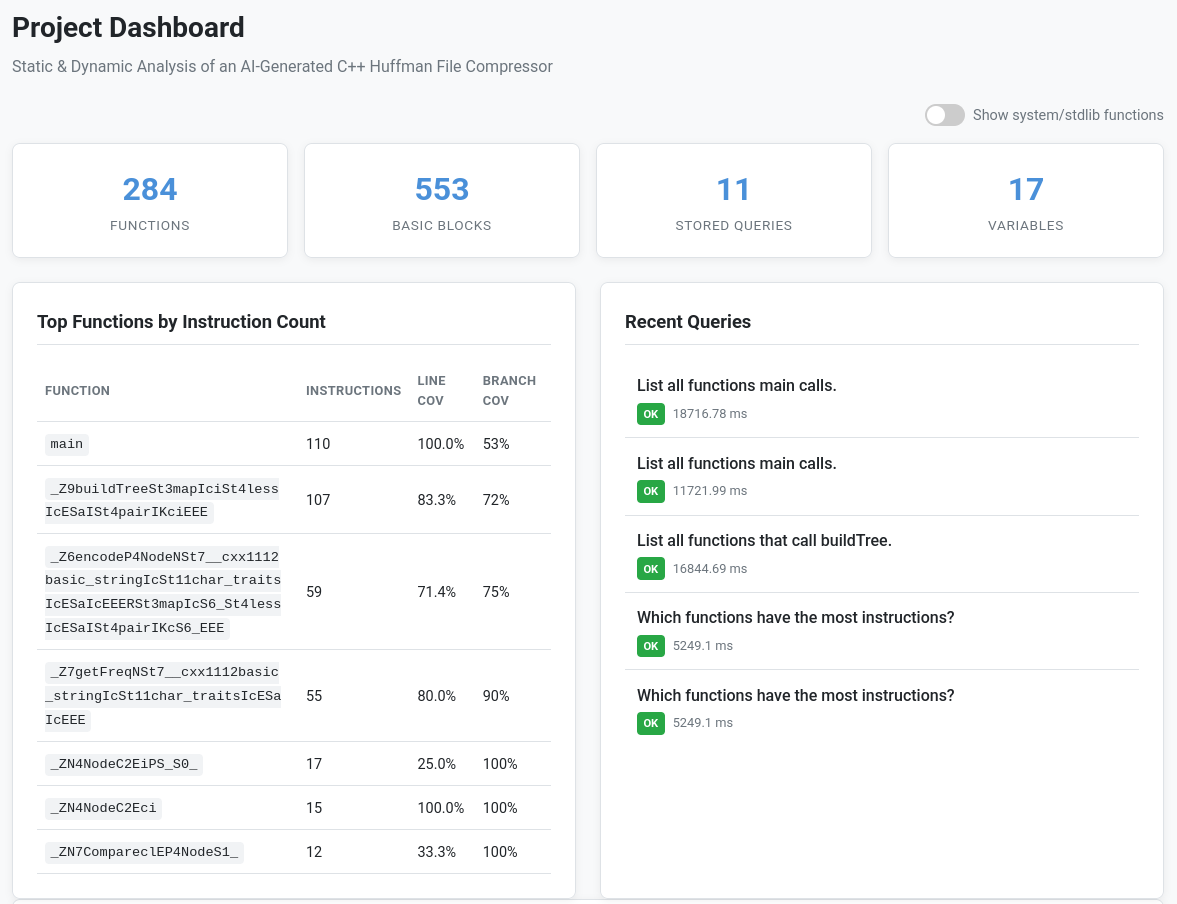
\includegraphics[width=0.95\textwidth]{screenshots/screenshot_query_log.png}
\end{figure}

\pagebreak

\section{Examples}

\textbf{Q1:} ``Show functions with branch coverage below 80 percent.''\\
\verb|MATCH (f:Function) WHERE f.branch_cov < 80 RETURN DISTINCT f.name|\\
Result: 280 functions (mostly STL internals at 0\%).

\begin{figure}[H]
\centering
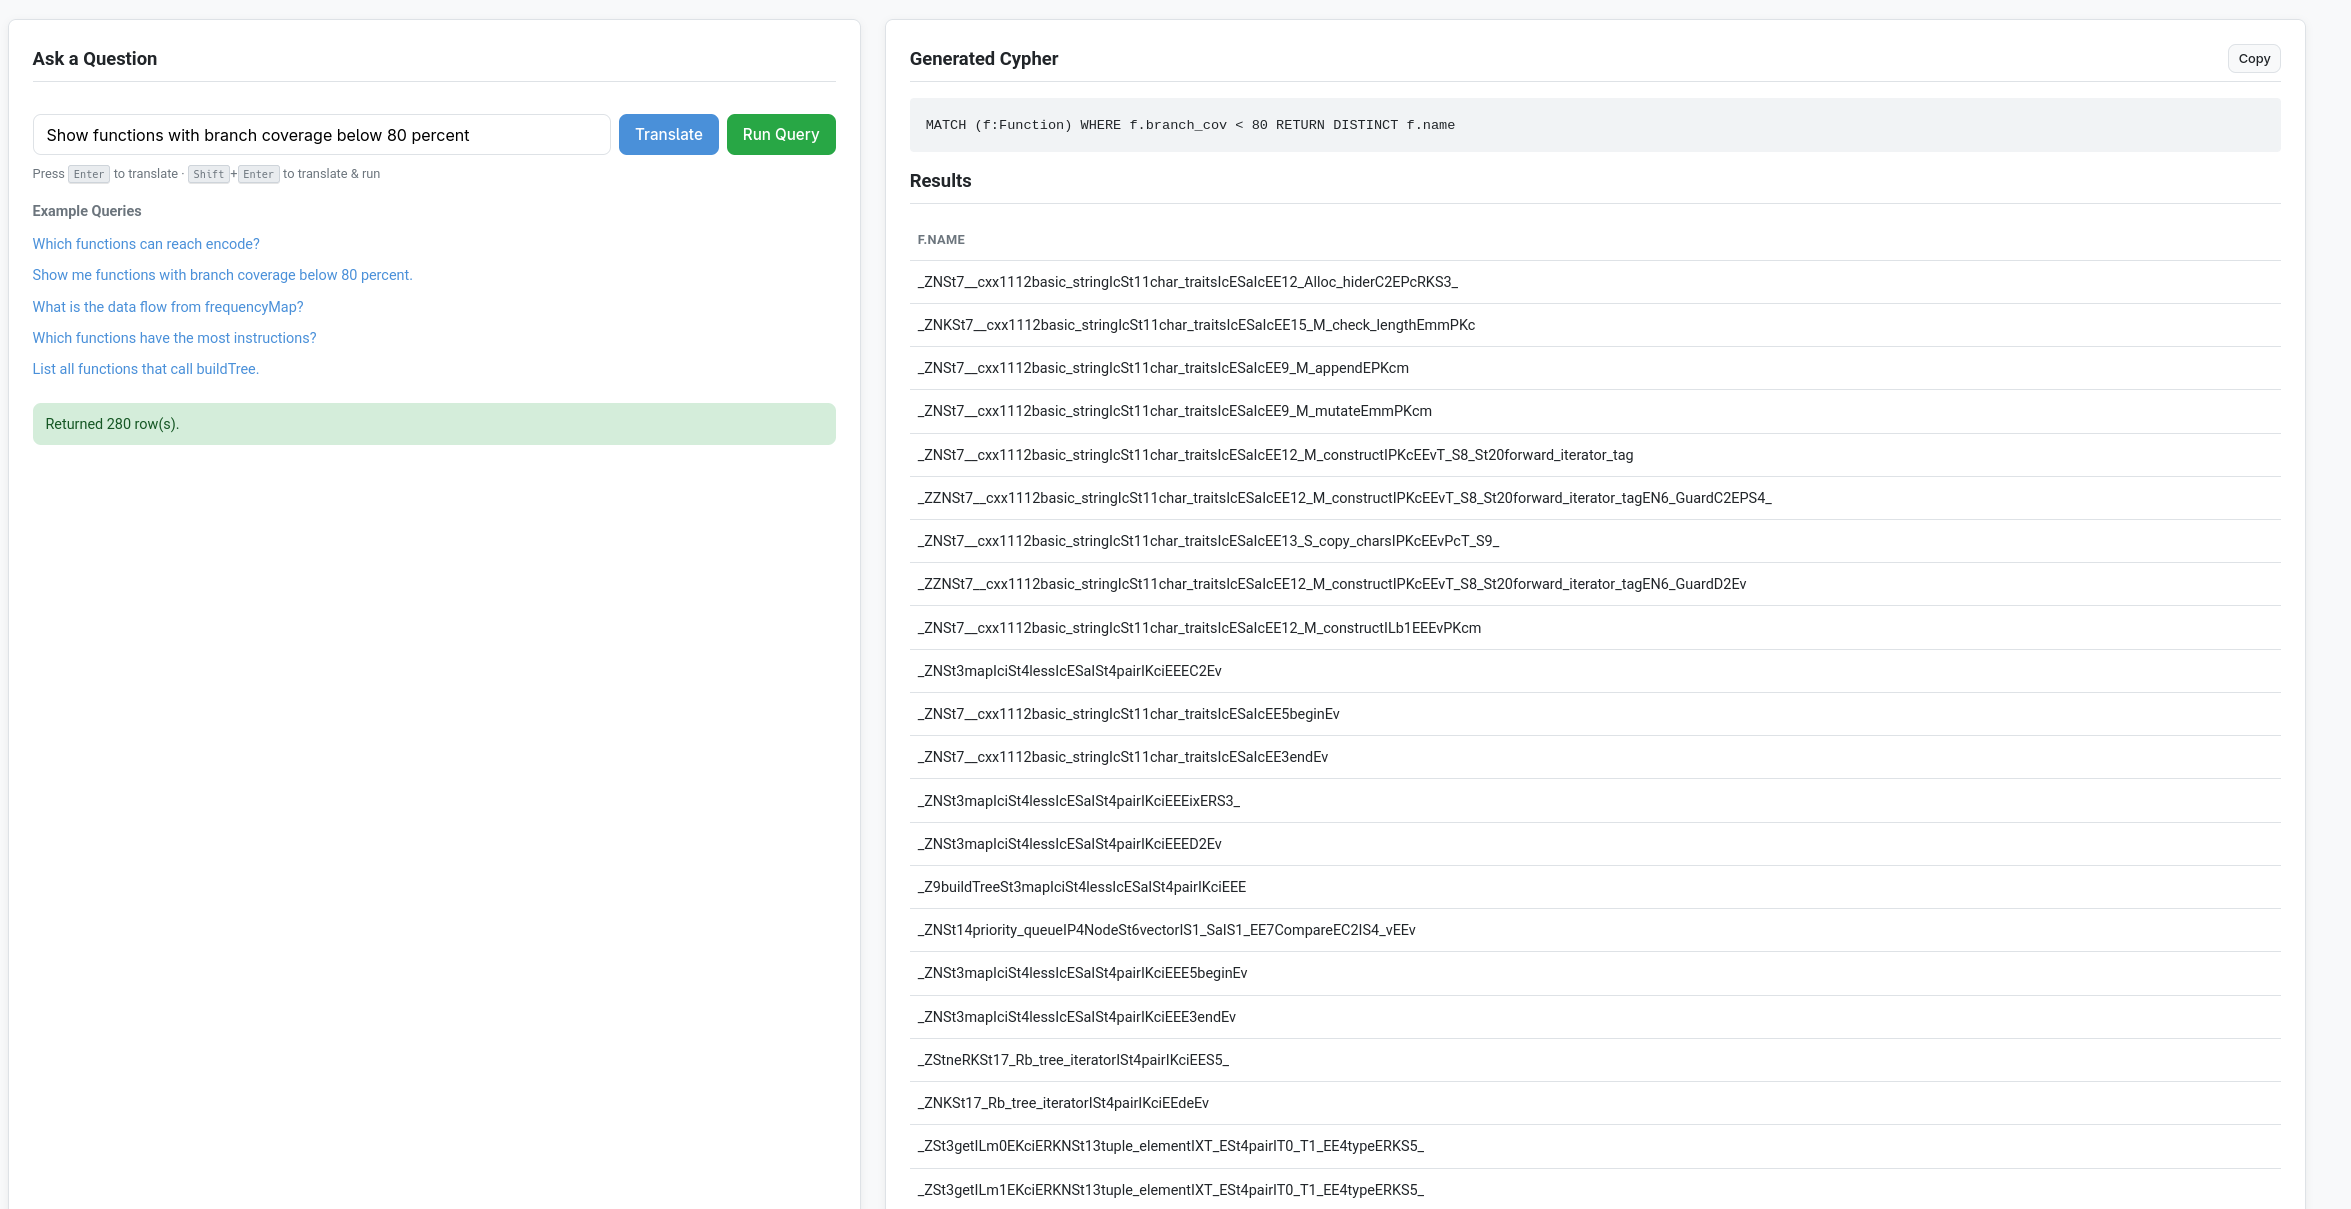
\includegraphics[width=0.95\textwidth]{screenshots/screenshot_query1_coverage.png}
\end{figure}

\noindent
\textbf{Q2:} ``Which functions can reach encode?''\\
\verb|MATCH (f:Function)-[:CALLS*]->(g:Function {name: 'encode'}) RETURN DISTINCT f.name|\\
Result: \texttt{main} (via getFreq $\rightarrow$ buildTree $\rightarrow$ encode).

\begin{figure}[H]
\centering
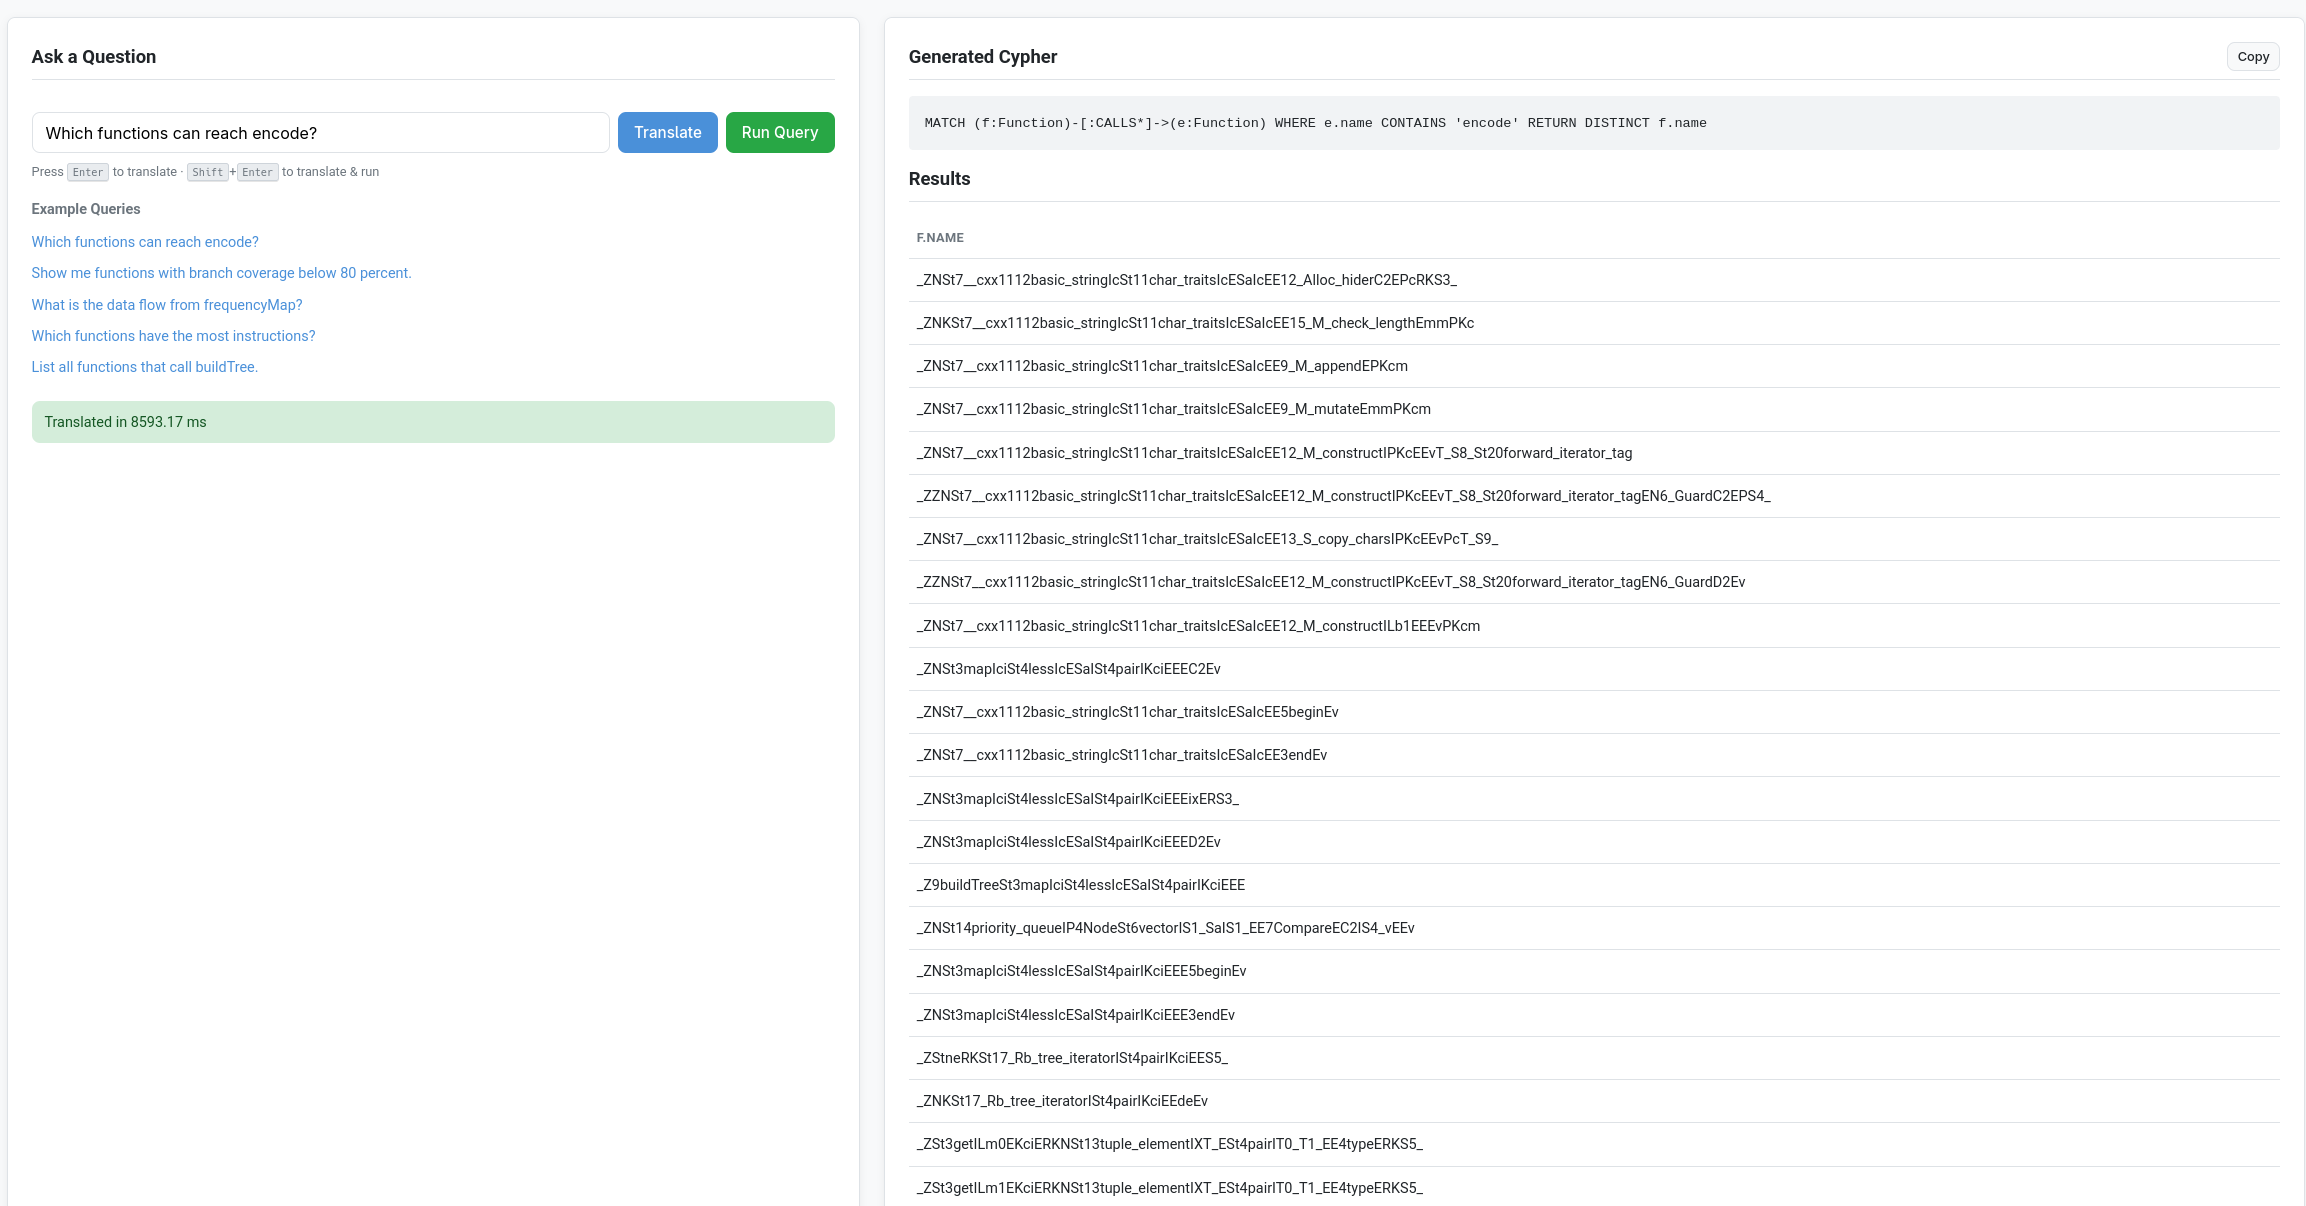
\includegraphics[width=0.95\textwidth]{screenshots/screenshot_query2_callgraph.png}
\end{figure}

\noindent
\textbf{Q3:} ``What is the data flow from main:freq?''\\
\verb|MATCH (v:Variable {name: 'main:freq'})-[:DEPENDS_ON]->(dep) RETURN dep.name|\\
Result: \texttt{getFreq:return}.

\begin{figure}[H]
\centering
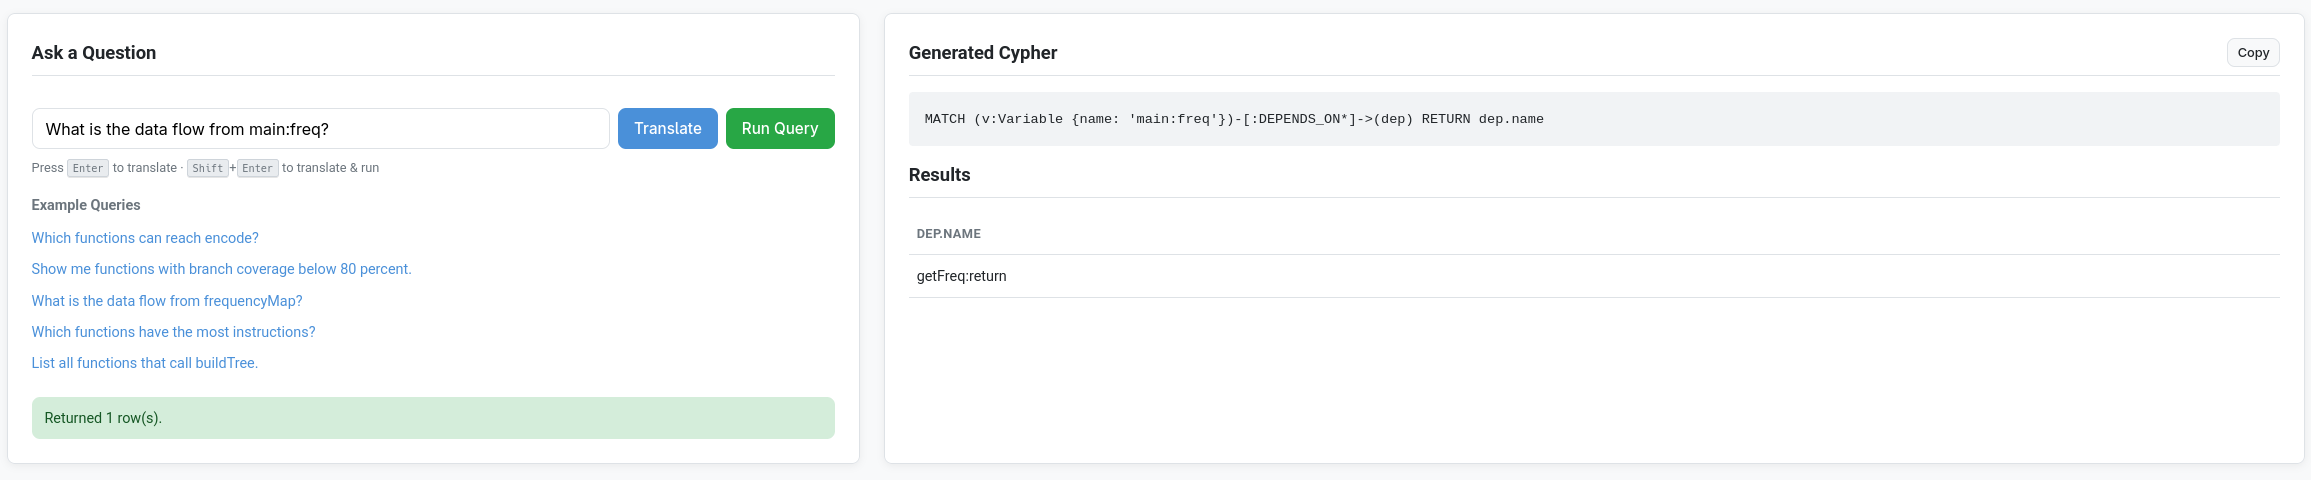
\includegraphics[width=0.95\textwidth]{screenshots/screenshot_query3_dataflow.png}
\end{figure}

\section{Extras}

\textbf{Auto-correction:} Hallucinated names (e.g., ``frequencyMap'') fuzzy-matched to valid names (e.g., ``main:freq'').\\
\textbf{Call Graph Viz:} Interactive D3.js force-directed graph.\\
\textbf{Function Explorer:} Table of 284 functions with static + dynamic metrics; modal shows callers, callees, CFG.

\begin{figure}[H]
\centering
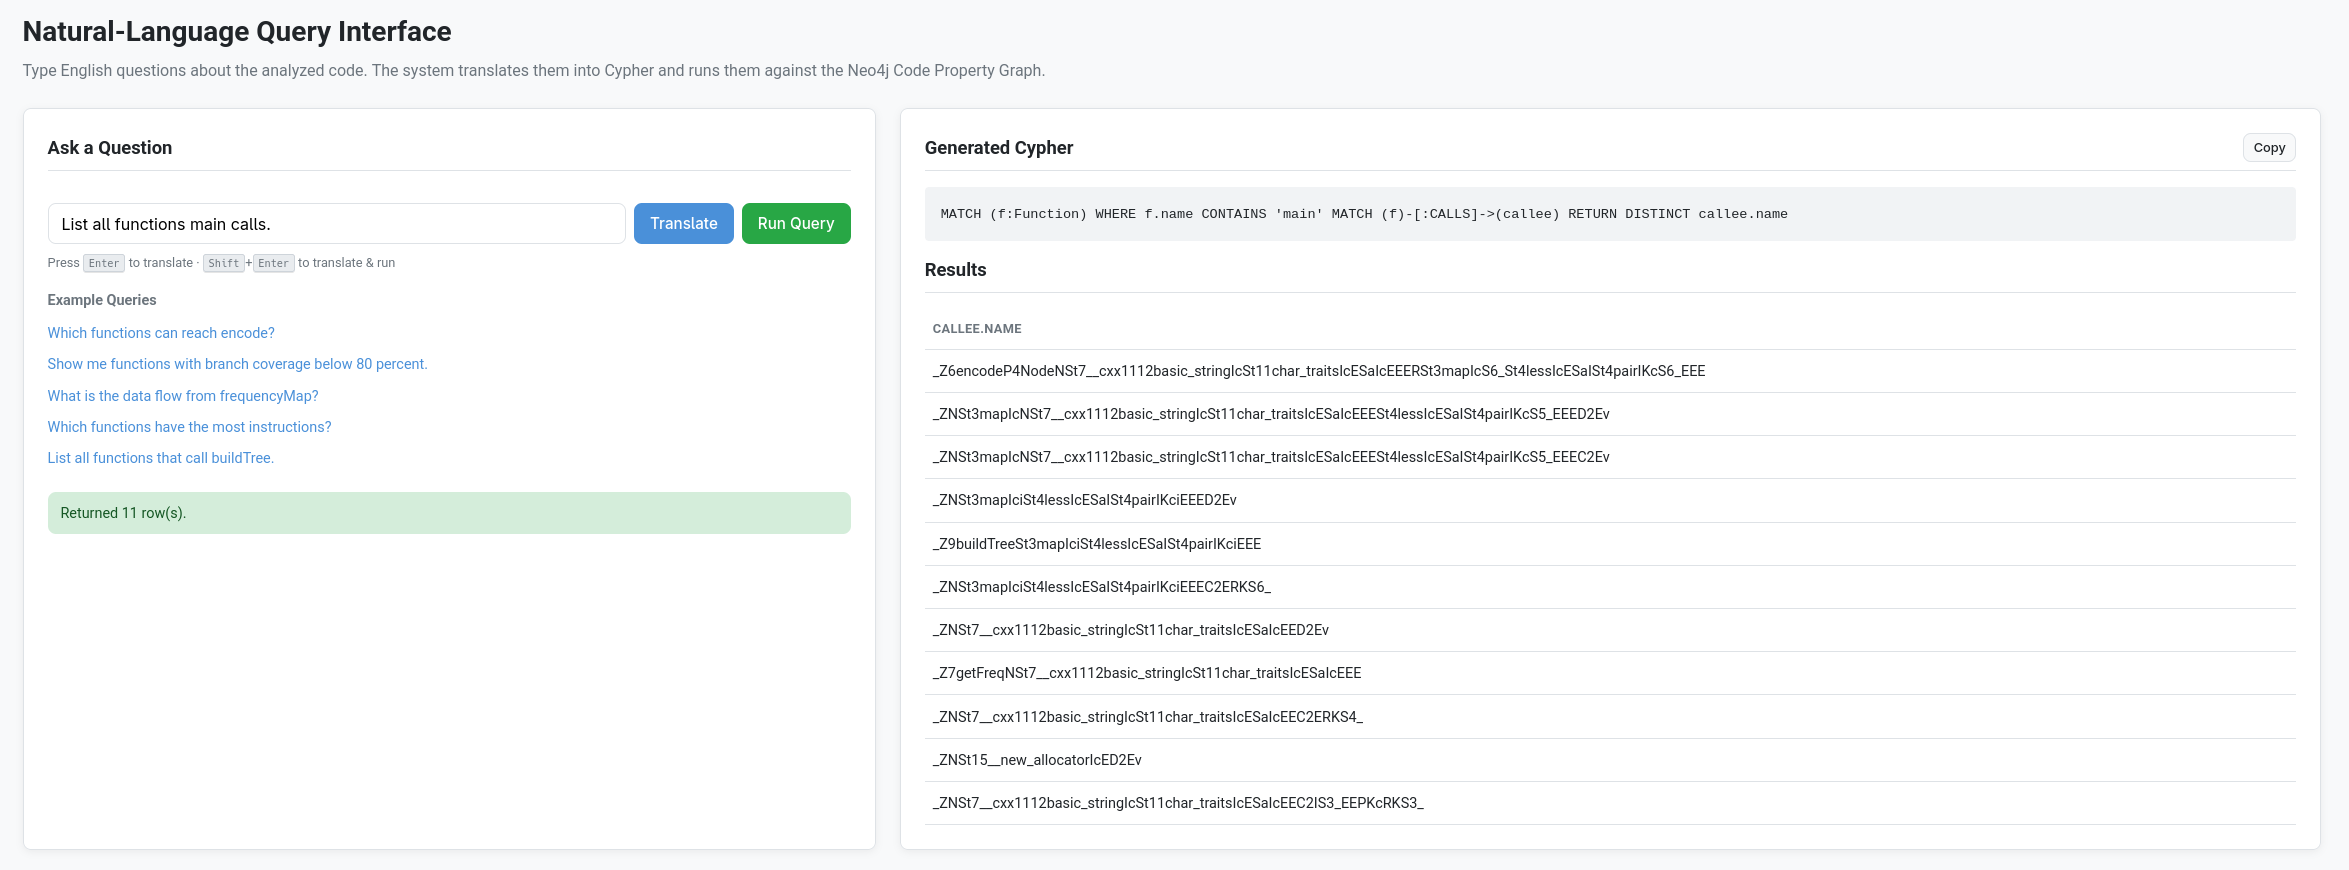
\includegraphics[width=0.95\textwidth]{screenshots/screenshot_call_result.png}
\end{figure}

\end{document}
